\pgfplotsset{compat=1.5}
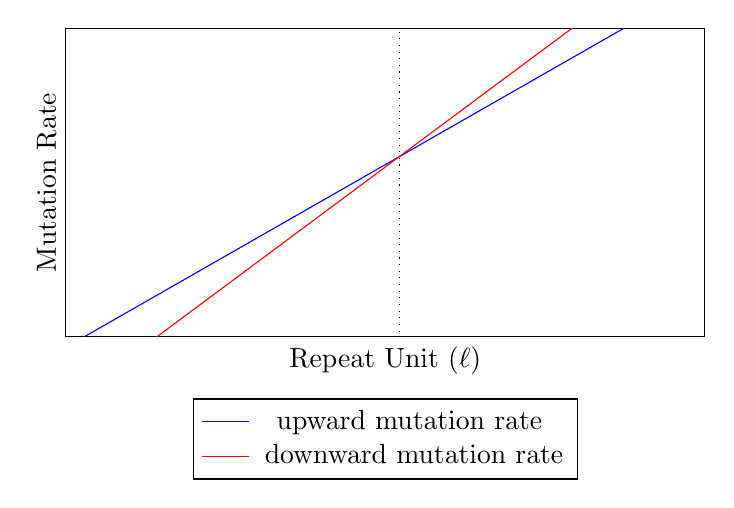
\begin{tikzpicture}
    \begin{axis}[
    width=0.8\linewidth, height=5.5cm,
    ylabel={Mutation Rate}, ymin=0.01, ymax=0.03,
    xlabel={Repeat Unit ($\ell$)}, xmin=2, xmax=13,
    xtick={0, 2, 4, 6, 8, 10, 12, 14, 16, 18, 20, 22, 24, 26},
    samples=100, no markers, enlargelimits=false, legend style={at={(0.5,-0.2)},anchor=north},
    domain=0:25, ticks=none
    ]
        \addplot {(0.0028/1.3)*x + 0.005};
        \addlegendentry{upward mutation rate};

        \addplot {0.0028*x};
        \addlegendentry{\vspace*{1em} downward mutation rate};

        \addplot+[mark=very thick, black, dotted, forget plot] coordinates {(7.7381, 0) (7.7381, 0.05)};
    \end{axis}
\end{tikzpicture}